\documentclass[tikz,border=0pt]{standalone}
\usepackage{xcolor}
\usetikzlibrary{calc}
% Palette: Sam_Comm_final.png by eye (vagrancy repository).
\definecolor{ink}{HTML}{3B2340}
\definecolor{dark}{HTML}{4A3357}
\definecolor{darkhi}{HTML}{5E4A6E}
\definecolor{sky}{HTML}{EFC46A}
\definecolor{skyhi}{HTML}{F5DA92}
\definecolor{skylow}{HTML}{E9B060}
\definecolor{cloud}{HTML}{F2D58A}
\definecolor{wallA}{HTML}{E88A73}
\definecolor{wallB}{HTML}{EE9F7E}
\definecolor{wallC}{HTML}{E47A7E}
\definecolor{wallD}{HTML}{F0B07E}
\definecolor{wallE}{HTML}{D9765F}
\definecolor{wallF}{HTML}{E99A8A}
\definecolor{greenA}{HTML}{8DBB7E}
\definecolor{greenB}{HTML}{6FA77A}
\definecolor{greenC}{HTML}{A9C97F}
\definecolor{greenD}{HTML}{5E9C6A}
\definecolor{window}{HTML}{F6E7A0}
\definecolor{windark}{HTML}{8C5A64}
\definecolor{plum}{HTML}{8A5A9E}
\definecolor{plumhi}{HTML}{A77BB8}
\definecolor{lilac}{HTML}{D9C3E0}
\definecolor{coral}{HTML}{E47A7E}
\definecolor{coraldk}{HTML}{C85F65}
\definecolor{orange}{HTML}{F26B38}
\definecolor{salmon}{HTML}{F4BE9C}
\definecolor{gold}{HTML}{F2B53A}
\definecolor{golddk}{HTML}{D9962A}
\definecolor{butter}{HTML}{F5DA92}
\definecolor{cream}{HTML}{FFF4E0}
\definecolor{paper}{HTML}{F6E7C4}
\definecolor{sage}{HTML}{8DBB7E}
\definecolor{sagedk}{HTML}{6FA77A}
\definecolor{forest}{HTML}{5E9C6A}
\definecolor{mint}{HTML}{C5E0B4}
\definecolor{teal}{HTML}{5FA8A0}
\definecolor{glass}{HTML}{A9D3C9}
\definecolor{glassdk}{HTML}{7FB7B0}
\definecolor{pink}{HTML}{F2A7B5}
\definecolor{rosewall}{HTML}{F3B7A8}
\definecolor{steel}{HTML}{C8C2B4}
\definecolor{steeldk}{HTML}{8D9A93}
\definecolor{metal}{HTML}{8D9A93}
\definecolor{wood}{HTML}{B9835A}
\definecolor{wooddk}{HTML}{8E5E3C}
\definecolor{tan}{HTML}{E2BD8C}
\definecolor{paving}{HTML}{E2BD8C}
\definecolor{ground}{HTML}{D3A77D}
% One ink for every outline.
\newcommand{\Ink}{1.3pt}
\tikzset{inked/.style={draw=ink, line width=\Ink, line join=round, line cap=round}}
% Picture units: 0.4 mm, y counted downward (hence the negative y unit).
\tikzset{x=0.4mm, y=-0.4mm}
\begin{document}
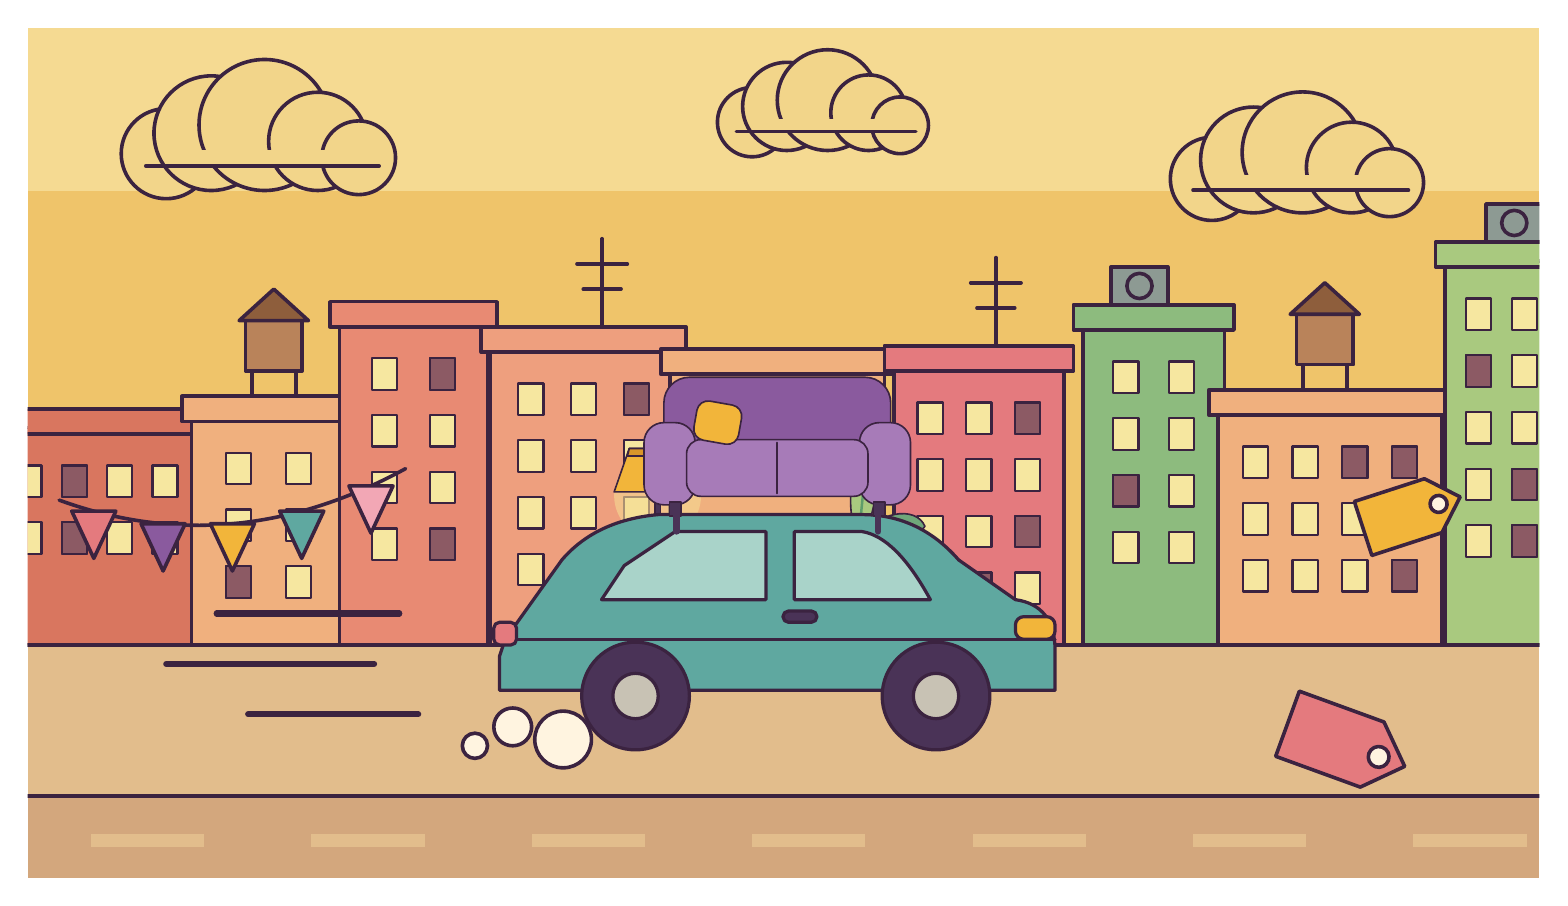
\begin{tikzpicture}
\clip (0,0) rectangle (480,270);
% sky and clouds
\fill[sky] (0,0) rectangle (480,270);
\fill[skyhi] (0,0) rectangle (480,52);
\filldraw[inked,fill=cloud] (44,40) circle [radius=14.3];
\filldraw[inked,fill=cloud] (58.3,33.5) circle [radius=18.2];
\filldraw[inked,fill=cloud] (75.2,30.9) circle [radius=20.8];
\filldraw[inked,fill=cloud] (92.1,36.1) circle [radius=15.6];
\filldraw[inked,fill=cloud] (105.1,41.3) circle [radius=11.7];
\fill[cloud] (44,38.7) rectangle (105.1,43.9);
\draw[ink, line width=1.3pt, line cap=round, line join=round] (37.5,43.9) -- (111.6,43.9);
\filldraw[inked,fill=cloud] (230,30) circle [radius=11];
\filldraw[inked,fill=cloud] (241,25) circle [radius=14];
\filldraw[inked,fill=cloud] (254,23) circle [radius=16];
\filldraw[inked,fill=cloud] (267,27) circle [radius=12];
\filldraw[inked,fill=cloud] (277,31) circle [radius=9];
\fill[cloud] (230,29) rectangle (277,33);
\draw[ink, line width=1.3pt, line cap=round, line join=round] (225,33) -- (282,33);
\filldraw[inked,fill=cloud] (376,48) circle [radius=13.2];
\filldraw[inked,fill=cloud] (389.2,42) circle [radius=16.8];
\filldraw[inked,fill=cloud] (404.8,39.6) circle [radius=19.2];
\filldraw[inked,fill=cloud] (420.4,44.4) circle [radius=14.4];
\filldraw[inked,fill=cloud] (432.4,49.2) circle [radius=10.8];
\fill[cloud] (376,46.8) rectangle (432.4,51.6);
\draw[ink, line width=1.3pt, line cap=round, line join=round] (370,51.6) -- (438.4,51.6);
% buildings
\filldraw[inked,fill=wallE] (-10,127) rectangle (54,196);
\filldraw[inked,fill=wallE] (-13,121) rectangle (57,129);
\foreach \i in {0,...,3} \foreach \j in {0,...,1} \filldraw[inked, line width=0.8pt, fill=window] (-3.6+\i*14.4,139+\j*18) rectangle ++(8,10);
\filldraw[inked, line width=0.8pt, fill=windark] (10.8,157) rectangle ++(8,10);
\filldraw[inked, line width=0.8pt, fill=windark] (10.8,139) rectangle ++(8,10);
\filldraw[inked,fill=wallD] (52,123) rectangle (101,196);
\filldraw[inked,fill=wallD] (49,117) rectangle (104,125);
\foreach \i in {0,...,1} \foreach \j in {0,...,2} \filldraw[inked, line width=0.8pt, fill=window] (63+\i*19,135+\j*18) rectangle ++(8,10);
\filldraw[inked, line width=0.8pt, fill=windark] (63,171) rectangle ++(8,10);
\draw[ink, line width=1.3pt, line cap=round, line join=round] (71.15,117) -- (71.15,109) (85.15,117) -- (85.15,109);
\filldraw[inked,fill=wood] (69.15,93) rectangle (87.15,109);
\filldraw[inked,fill=wooddk] (67.15,93) -- (78.15,83) -- (89.15,93) -- cycle;
\filldraw[inked,fill=wallA] (99,93) rectangle (146,196);
\filldraw[inked,fill=wallA] (96,87) rectangle (149,95);
\foreach \i in {0,...,1} \foreach \j in {0,...,3} \filldraw[inked, line width=0.8pt, fill=window] (109.33+\i*18.33,105+\j*18) rectangle ++(8,10);
\filldraw[inked, line width=0.8pt, fill=windark] (127.67,159) rectangle ++(8,10);
\filldraw[inked, line width=0.8pt, fill=windark] (127.67,105) rectangle ++(8,10);
\filldraw[inked,fill=wallB] (147,101) rectangle (206,196);
\filldraw[inked,fill=wallB] (144,95) rectangle (209,103);
\foreach \i in {0,...,2} \foreach \j in {0,...,3} \filldraw[inked, line width=0.8pt, fill=window] (155.75+\i*16.75,113+\j*18) rectangle ++(8,10);
\filldraw[inked, line width=0.8pt, fill=windark] (172.5,167) rectangle ++(8,10);
\filldraw[inked, line width=0.8pt, fill=windark] (189.25,167) rectangle ++(8,10);
\filldraw[inked, line width=0.8pt, fill=windark] (189.25,113) rectangle ++(8,10);
\draw[ink, line width=1.3pt, line cap=round, line join=round] (182.4,95) -- (182.4,67) (174.4,75) -- (190.4,75) (176.4,83) -- (188.4,83);
\filldraw[inked,fill=wallD] (204,108) rectangle (272,196);
\filldraw[inked,fill=wallD] (201,102) rectangle (275,110);
\foreach \i in {0,...,3} \foreach \j in {0,...,3} \filldraw[inked, line width=0.8pt, fill=window] (211.2+\i*15.2,120+\j*18) rectangle ++(8,10);
\filldraw[inked, line width=0.8pt, fill=windark] (211.2,174) rectangle ++(8,10);
\filldraw[inked, line width=0.8pt, fill=windark] (226.4,120) rectangle ++(8,10);
\filldraw[inked, line width=0.8pt, fill=windark] (241.6,138) rectangle ++(8,10);
\filldraw[inked, line width=0.8pt, fill=windark] (241.6,120) rectangle ++(8,10);
\filldraw[inked,fill=wallC] (275,107) rectangle (329,196);
\filldraw[inked,fill=wallC] (272,101) rectangle (332,109);
\foreach \i in {0,...,2} \foreach \j in {0,...,3} \filldraw[inked, line width=0.8pt, fill=window] (282.5+\i*15.5,119+\j*18) rectangle ++(8,10);
\filldraw[inked, line width=0.8pt, fill=windark] (313.5,155) rectangle ++(8,10);
\filldraw[inked, line width=0.8pt, fill=windark] (313.5,119) rectangle ++(8,10);
\filldraw[inked, line width=0.8pt, fill=windark] (298,173) rectangle ++(8,10);
\draw[ink, line width=1.3pt, line cap=round, line join=round] (307.4,101) -- (307.4,73) (299.4,81) -- (315.4,81) (301.4,89) -- (313.4,89);
\filldraw[inked,fill=greenA] (335,94) rectangle (380,196);
\filldraw[inked,fill=greenA] (332,88) rectangle (383,96);
\foreach \i in {0,...,1} \foreach \j in {0,...,3} \filldraw[inked, line width=0.8pt, fill=window] (344.67+\i*17.67,106+\j*18) rectangle ++(8,10);
\filldraw[inked, line width=0.8pt, fill=windark] (344.67,142) rectangle ++(8,10);
\filldraw[inked, line width=0.8pt, fill=windark] (344.67,142) rectangle ++(8,10);
\filldraw[inked,fill=metal] (344,76) rectangle (362,88);
\filldraw[inked,fill=steeldk] (353,82) circle [radius=4];
\filldraw[inked,fill=wallD] (378,121) rectangle (449,196);
\filldraw[inked,fill=wallD] (375,115) rectangle (452,123);
\foreach \i in {0,...,3} \foreach \j in {0,...,2} \filldraw[inked, line width=0.8pt, fill=window] (385.8+\i*15.8,133+\j*18) rectangle ++(8,10);
\filldraw[inked, line width=0.8pt, fill=windark] (417.4,133) rectangle ++(8,10);
\filldraw[inked, line width=0.8pt, fill=windark] (433.2,169) rectangle ++(8,10);
\filldraw[inked, line width=0.8pt, fill=windark] (433.2,133) rectangle ++(8,10);
\draw[ink, line width=1.3pt, line cap=round, line join=round] (404.85,115) -- (404.85,107) (418.85,115) -- (418.85,107);
\filldraw[inked,fill=wood] (402.85,91) rectangle (420.85,107);
\filldraw[inked,fill=wooddk] (400.85,91) -- (411.85,81) -- (422.85,91) -- cycle;
\filldraw[inked,fill=greenC] (450,74) rectangle (515,196);
\filldraw[inked,fill=greenC] (447,68) rectangle (518,76);
\foreach \i in {0,...,3} \foreach \j in {0,...,4} \filldraw[inked, line width=0.8pt, fill=window] (456.6+\i*14.6,86+\j*18) rectangle ++(8,10);
\filldraw[inked, line width=0.8pt, fill=windark] (500.4,86) rectangle ++(8,10);
\filldraw[inked, line width=0.8pt, fill=windark] (471.2,158) rectangle ++(8,10);
\filldraw[inked, line width=0.8pt, fill=windark] (456.6,104) rectangle ++(8,10);
\filldraw[inked, line width=0.8pt, fill=windark] (471.2,140) rectangle ++(8,10);
\filldraw[inked, line width=0.8pt, fill=windark] (485.8,140) rectangle ++(8,10);
\filldraw[inked,fill=metal] (463,56) rectangle (481,68);
\filldraw[inked,fill=steeldk] (472,62) circle [radius=4];
% pavement
\fill[paving] (0,196) rectangle (480,270);
\draw[ink, line width=1.3pt, line cap=round, line join=round] (0,196) -- (480,196);
\fill[ground] (0,244) rectangle (480,270);
\draw[ink, line width=1.3pt, line cap=round, line join=round] (0,244) -- (480,244);
\foreach \dx in {20,90,...,480} \fill[tan] (\dx,256) rectangle ++(36,4);
% the car home, loaded: what pokes out of the windows goes in first
\begin{scope}[shift={(164,124)}, scale=0.3]
\renewcommand{\Ink}{0.59pt}
\filldraw[inked,fill=butter,draw=none,opacity=0.6] (120,82) circle [radius=46];
\filldraw[inked,fill=dark] (117,70) rectangle (123,152);
\filldraw[inked,fill=gold] (90,32) -- (150,32) -- (166,78) -- (74,78) -- cycle;
\filldraw[inked,fill=golddk] (90,32) -- (150,32) -- (152,40) -- (88,40) -- cycle;
\filldraw[inked,fill=dark] (120,152) ellipse [x radius=30, y radius=7];
\end{scope}
\begin{scope}[shift={(230,132)}, scale=0.28]
\renewcommand{\Ink}{0.59pt}
\filldraw[inked,fill=sage] (120,112) .. controls (100,80) and (60,70) .. (46,92) .. controls (58,112) and (96,118) .. (120,112) -- cycle;
\filldraw[inked,fill=sagedk] (120,112) .. controls (140,76) and (186,70) .. (196,94) .. controls (182,114) and (144,118) .. (120,112) -- cycle;
\filldraw[inked,fill=greenC] (120,112) .. controls (106,70) and (110,32) .. (130,20) .. controls (148,46) and (138,88) .. (120,112) -- cycle;
\draw[forest, line width=0.9pt, line cap=round, line join=round] (70,92) -- (104,106) (168,90) -- (138,106) (128,34) -- (122,96);
\filldraw[inked,fill=coral] (88,112) -- (152,112) -- (142,156) -- (98,156) -- cycle;
\filldraw[inked,fill=coraldk,rounded corners=0.45mm] (84,106) rectangle (156,119);
\end{scope}
\begin{scope}[shift={(130,88)}, scale=0.9]
\renewcommand{\Ink}{1.17pt}
\filldraw[inked,fill=teal] (24,118) -- (44,90) .. controls (52,80.67) and (63.33,75.33) .. (78,74) -- (150,74) .. controls (163.33,74) and (174.67,79.33) .. (184,90) -- (204,104) .. controls (213.33,105.33) and (218,111.33) .. (218,122) -- (218,136) -- (22,136) -- (22,124) -- cycle;
\filldraw[inked,fill=glass] (66,92) -- (84,80) -- (116,80) -- (116,104) -- (58,104) -- cycle;
\filldraw[inked,fill=glass] (126,80) -- (150,80) .. controls (158,81.33) and (166,89.33) .. (174,104) -- (126,104) -- cycle;
\draw[ink, line width=1.17pt, line cap=round, line join=round] (24,118) -- (218,118);
\filldraw[inked,fill=dark,rounded corners=0.72mm] (122,108) rectangle (134,112);
\filldraw[inked,fill=gold,rounded corners=1.08mm] (204,110) rectangle (218,118);
\filldraw[inked,fill=coral,rounded corners=0.72mm] (20,112) rectangle (28,120);
\filldraw[inked,fill=dark] (70,138) circle [radius=19];
\filldraw[inked,fill=steel] (70,138) circle [radius=8];
\filldraw[inked,fill=dark] (176,138) circle [radius=19];
\filldraw[inked,fill=steel] (176,138) circle [radius=8];
\end{scope}
\begin{scope}[shift={(184,84)}, scale=0.45]
\renewcommand{\Ink}{0.59pt}
\filldraw[inked,fill=plum,rounded corners=3.24mm] (40,60) rectangle (200,118);
\filldraw[inked,fill=plumhi,rounded corners=2.52mm] (26,92) rectangle (62,150);
\filldraw[inked,fill=plumhi,rounded corners=2.52mm] (178,92) rectangle (214,150);
\filldraw[inked,fill=plumhi,rounded corners=1.8mm] (56,104) rectangle (184,144);
\draw[ink, line width=0.59pt, line cap=round, line join=round] (120,106) -- (120,142);
\begin{scope}[shift={(0,0)}, rotate around={-10:(78,92)}]
\filldraw[inked,fill=gold,rounded corners=1.44mm] (62,78) rectangle (94,106);
\end{scope}
\filldraw[inked,fill=dark] (44,148) rectangle (52,158);
\filldraw[inked,fill=dark] (188,148) rectangle (196,158);
\end{scope}
\draw[dark, line width=2.2pt, line cap=round, line join=round] (206,152) -- (206,160) (270,152) -- (270,160);
% speed lines and dust
\draw[ink, line width=2.2pt, line cap=round, line join=round] (60,186) -- (118,186) (44,202) -- (110,202) (70,218) -- (124,218);
\filldraw[inked,fill=cream] (170,226) circle [radius=9];
\filldraw[inked,fill=cream] (154,222) circle [radius=6];
\filldraw[inked,fill=cream] (142,228) circle [radius=4];
\draw[ink, line width=1.3pt, line cap=round, line join=round] (10,150) .. controls (46.67,163.33) and (83.33,160) .. (120,140);
\filldraw[inked,fill=coral] (14,153.5) -- (28,153.5) -- (21,168.5) -- cycle;
\filldraw[inked,fill=plum] (36,157.5) -- (50,157.5) -- (43,172.5) -- cycle;
\filldraw[inked,fill=gold] (58,157.5) -- (72,157.5) -- (65,172.5) -- cycle;
\filldraw[inked,fill=teal] (80,153.5) -- (94,153.5) -- (87,168.5) -- cycle;
\filldraw[inked,fill=pink] (102,145.5) -- (116,145.5) -- (109,160.5) -- cycle;
\begin{scope}[shift={(400,210)}, scale=1.1, rotate around={-20:(0,10)}]
\filldraw[inked,fill=coral] (0,0) -- (26,0) -- (36,10) -- (26,20) -- (0,20) -- cycle;
\filldraw[inked,fill=cream] (28,10) circle [radius=3];
\end{scope}
\begin{scope}[shift={(424,150)}, scale=0.9, rotate around={18:(0,10)}]
\filldraw[inked,fill=gold] (0,0) -- (26,0) -- (36,10) -- (26,20) -- (0,20) -- cycle;
\filldraw[inked,fill=cream] (28,10) circle [radius=3];
\end{scope}
\end{tikzpicture}
\end{document}
